\documentclass[tikz,border=8pt]{standalone}
\usepackage{amsmath,amssymb}
\usetikzlibrary{arrows.meta,calc}

\begin{document}
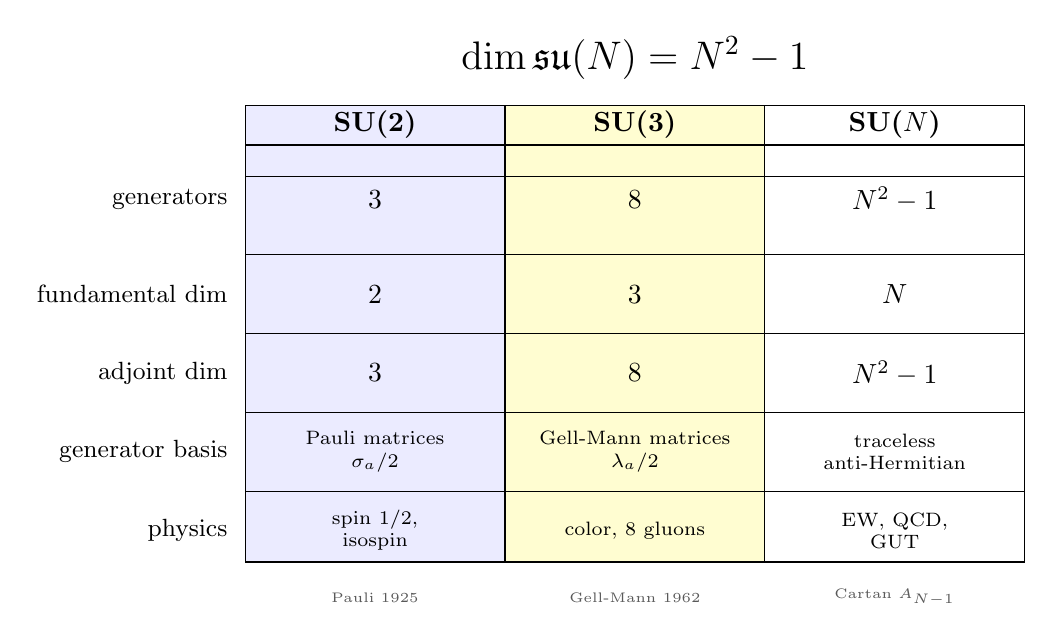
\begin{tikzpicture}[>=Latex]

  % Title
  \node[font=\Large] at (4.95, 5) {$\dim\mathfrak{su}(N)=N^2-1$};

  % Column backgrounds
  \fill[blue!8]    (0, -1.4) rectangle (3.3, 4.4);
  \fill[yellow!18] (3.3, -1.4) rectangle (6.6, 4.4);
  \fill[white]     (6.6, -1.4) rectangle (9.9, 4.4);

  % Grid
  \draw[thin] (0, -1.4) rectangle (9.9, 4.4);
  \draw[thin] (3.3, -1.4) -- (3.3, 4.4);
  \draw[thin] (6.6, -1.4) -- (6.6, 4.4);
  \foreach \y in {3.5, 2.5, 1.5, 0.5, -0.5}{
    \draw[thin] (0, \y) -- (9.9, \y);
  }
  \draw[thick] (0, 3.9) -- (9.9, 3.9);

  % Headers
  \node[font=\bfseries] at (1.65, 4.15) {SU(2)};
  \node[font=\bfseries] at (4.95, 4.15) {SU(3)};
  \node[font=\bfseries] at (8.25, 4.15) {SU($N$)};

  % Row labels (left, outside)
  \node[font=\small, anchor=east] at (-0.1, 3.2) {generators};
  \node[font=\small, anchor=east] at (-0.1, 2.0) {fundamental dim};
  \node[font=\small, anchor=east] at (-0.1, 1.0) {adjoint dim};
  \node[font=\small, anchor=east] at (-0.1, 0.0) {generator basis};
  \node[font=\small, anchor=east] at (-0.1, -1.0) {physics};

  % Row 1: generators (3, 8, N^2-1)
  \node at (1.65, 3.2) {$3$};
  \node at (4.95, 3.2) {$8$};
  \node at (8.25, 3.2) {$N^2-1$};

  % Row 2: fundamental
  \node at (1.65, 2.0) {$2$};
  \node at (4.95, 2.0) {$3$};
  \node at (8.25, 2.0) {$N$};

  % Row 3: adjoint
  \node at (1.65, 1.0) {$3$};
  \node at (4.95, 1.0) {$8$};
  \node at (8.25, 1.0) {$N^2-1$};

  % Row 4: generator basis
  \node[font=\scriptsize, align=center] at (1.65, 0.0) {Pauli matrices\\$\sigma_a/2$};
  \node[font=\scriptsize, align=center] at (4.95, 0.0) {Gell-Mann matrices\\$\lambda_a/2$};
  \node[font=\scriptsize, align=center] at (8.25, 0.0) {traceless\\anti-Hermitian};

  % Row 5: physics
  \node[font=\scriptsize, align=center] at (1.65, -1.0) {spin 1/2,\\isospin};
  \node[font=\scriptsize, align=center] at (4.95, -1.0) {color, 8 gluons};
  \node[font=\scriptsize, align=center] at (8.25, -1.0) {EW, QCD,\\GUT};

  % Bottom credit
  \node[font=\tiny, gray!70!black] at (1.65, -1.85) {Pauli 1925};
  \node[font=\tiny, gray!70!black] at (4.95, -1.85) {Gell-Mann 1962};
  \node[font=\tiny, gray!70!black] at (8.25, -1.85) {Cartan $A_{N-1}$};
\end{tikzpicture}
\end{document}
